\documentclass[12pt]{article}

\usepackage[utf8]{inputenc}
\usepackage[T1]{fontenc}
\usepackage[spanish]{babel}
\usepackage{graphicx}
\usepackage{listings}
\usepackage{caption}
\usepackage{subcaption}
\usepackage[right=2cm,left=2cm,top=2cm,bottom=2cm]{geometry}
\usepackage{hyperref}
\usepackage{fancyhdr}
\usepackage{color}
\usepackage[export]{adjustbox}
\usepackage{graphicx}
\usepackage{float}
\usepackage{changepage}
\usepackage{multicol}
\usepackage{imakeidx}
\usepackage[spanish]{babel}
\usepackage[backend=biber]{biblatex}

\pagestyle{fancy}
\renewcommand{\footrulewidth}{0.4pt}
\setlength{\headheight}{15pt}


\fancyhead[L]{ CEIABD – MIA }
\fancyhead[R]{ Páez Anguita, Víctor }
\fancyfoot[L]{IES Gran Capitán}


\begin{document}

\begin{titlepage}
    \begin{center}
      \Large \bfseries{}
    \end{center}
    \vspace{0.1cm}
    \begin{center}
      \Large \bfseries{}
    \end{center}
    \vspace{0.1cm}
    \begin{center}
     \Large \bfseries{Actividad 2}
    \end{center}
    \vspace{0.0001cm}
    \begin{center}
        Departamento de informática \\ I.E.S. Gran Capitán - Córdoba
    \end{center}
        \vspace{2 cm}
\begin{figure}[h!]
    \centering
    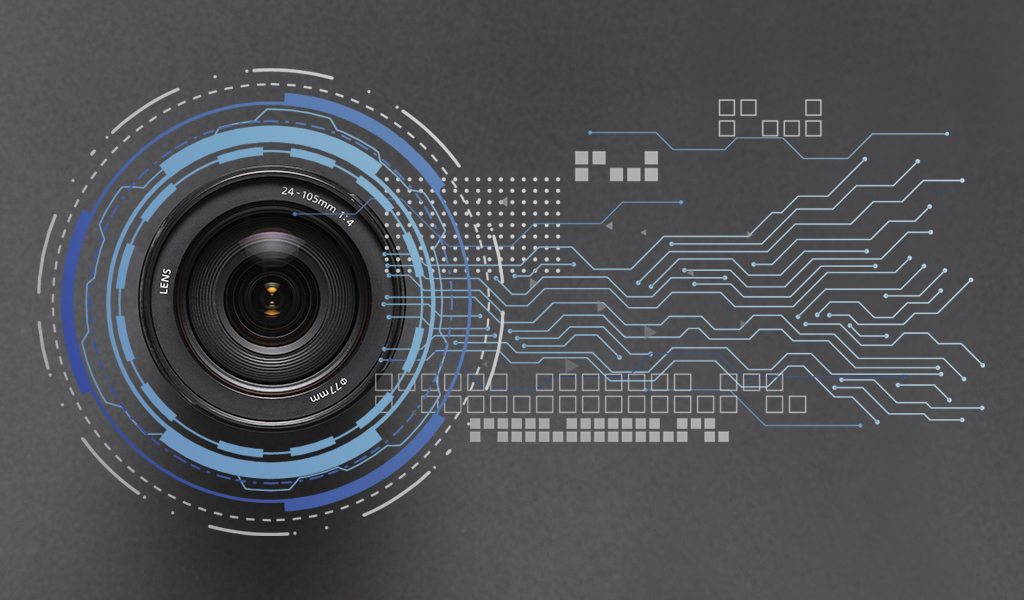
\includegraphics[width=.8\textwidth]{visión-artificial.jpg}
    \label{fig:my_label}
\end{figure}
    \vspace{0.2 cm}
    \begin{center}
        Inteligencia artificial y Big data \\ Córdoba, 14 de Octubre 2024
    \end{center}
    \vspace{4 cm}
\null\hfill \textbf{Desarrollado por:}
\\
\\
\null\hfill Víctor Páez Anguita
\clearpage
\end{titlepage}

%%%%%%%%%%%%%%%%%%%%%%%%%%%Index%%%%%%%%%%%%%%%%%%%%%%%%%%%%%%%%
\tableofcontents
\clearpage
%%%%%%%%%%%%%%%%%%%%%%%%%%%Index%%%%%%%%%%%%%%%%%%%%%%%%%%%%%%%%

\section{Introducción}
En esta actividad veremos ejemplos de distintas aplicaciones que se le pueden dar a la visión artificial. En la industria del cine, aplicaciones industriales, en el día a día, etc.

\section{Aplicación de la visión artifical}

\subsection{Industria del cine}

En el cine, la visión artificial juega un papel importante en la realidad aumentada y virtual. Permite crear efectos visuales precisos y modelados 3D a partir de imágenes bidimensionales, 
usados para mejorar las experiencias inmersivas en películas y videojuegos. También se emplea en seguimiento de movimiento, 
donde se capturan y analizan las acciones de actores reales para animar personajes digitales de forma más realista.

\subsection{Aplicaciones industriales}

Control de calidad: En sectores como la automoción y electrónica, se utiliza la visión artificial para la inspección de productos. 
Se detectan defectos en las piezas en las etapas tempranas de producción, lo que mejora la eficiencia y la calidad del producto final.
\\
Robótica: Los robots industriales dependen de la visión artificial para navegar, manipular objetos y colaborar con humanos. 
Es fundamental en tareas de precisión como el ensamblaje o la soldadura.
\\
Monitoreo y mantenimiento: En fábricas, se utiliza para identificar señales de desgaste o anomalías en las máquinas, ayudando en el mantenimiento preventivo y reduciendo
costes por fallos inesperados.

\subsection{Vida Cotidiana y Social}

En la vida diaria, la visión artificial aparece en funciones como el reconocimiento facial en smartphones, facilitando el acceso seguro y personalizado. 
También se aplica en redes sociales y cámaras de vigilancia para mejorar la interacción y la seguridad.

\clearpage
\section{Otros usos}
\subsection{Agricultura}
En el sector agrícola, se utiliza para la detección de enfermedades en cultivos y para clasificar productos alimenticios como frutas y verduras, según su madurez o calidad.
\\
Por otra parte, también se puede utilizar para el escaneo de areas de cultivo. Con ello se puede delimitar en un mapa la propia area en custión para que posteriormente un dron pueda reconocer el area y
tratar de manera autonoma los cultivos en vez de utilizar tractores.

\subsection{Conducción autónoma}

Los vehículos autónomos, como los de Tesla y Waymo, usan la visión artificial para detectar el entorno, desde peatones hasta señales de tráfico. 
Esta tecnología es clave para evitar accidentes y mejorar la seguridad en carreteras.

\subsection{Diagnóstico Médico}

En medicina, la visión artificial se aplica en la interpretación de imágenes como radiografías y tomografías. Ayuda a los médicos a detectar anomalías, 
como tumores o enfermedades cardiovasculares, con gran precisión. También se utiliza en cirugías asistidas para proporcionar información visual detallada en tiempo real.
\clearpage

\section{Bibliografia}
\begin{itemize}
    \item \href{https://dezzai.com/es/blog/explorando-las-posibilidades-8-ejemplos-reales-de-vision-artificial/}{Articulo de dezzai}.
    \item \href{https://bcnvision.es/blog-vision-artificial/las-10-mejores-aplicaciones-de-vision-artificial-en-la-industria/}{Articulo de bncvision}
    \item \href{https://atriainnovation.com/blog/aplicaciones-de-la-vision-artificial-en-la-industria/}{Articulo atriainnovation}
\end{itemize}

\end{document}
